\documentclass{article}
\usepackage{mathtools}
\usepackage{graphicx}
\graphicspath{ {/} }
\title{Graph-based Data Model and Remote Monitoring for Electrical Microgrid Systems}
\author{Jake Billings}
\date{May 02, 2018}
\begin{document}
\maketitle

\section{Introduction}
A proposed alternative system for generation of electricity is the electrical microgrid. In a traditional electrical grid, utilities exploit economies of scale to separate power generation from power consumption. Very large generators are placed miles outside of cities, and high voltage electrical lines transport power long distances before it is consumed. Microgrid systems place smaller generators closer to sources of power usage. This reduces loss due to transmission and distributes risk of failure. However, it dramatically increases the complexity of control problems. This paper does not detail control systems for microgrids. However, it does propose a mathematical model and data gathering system that could be used to monitor microgrid systems.

\section{Model}


\subsection{Java Classes}
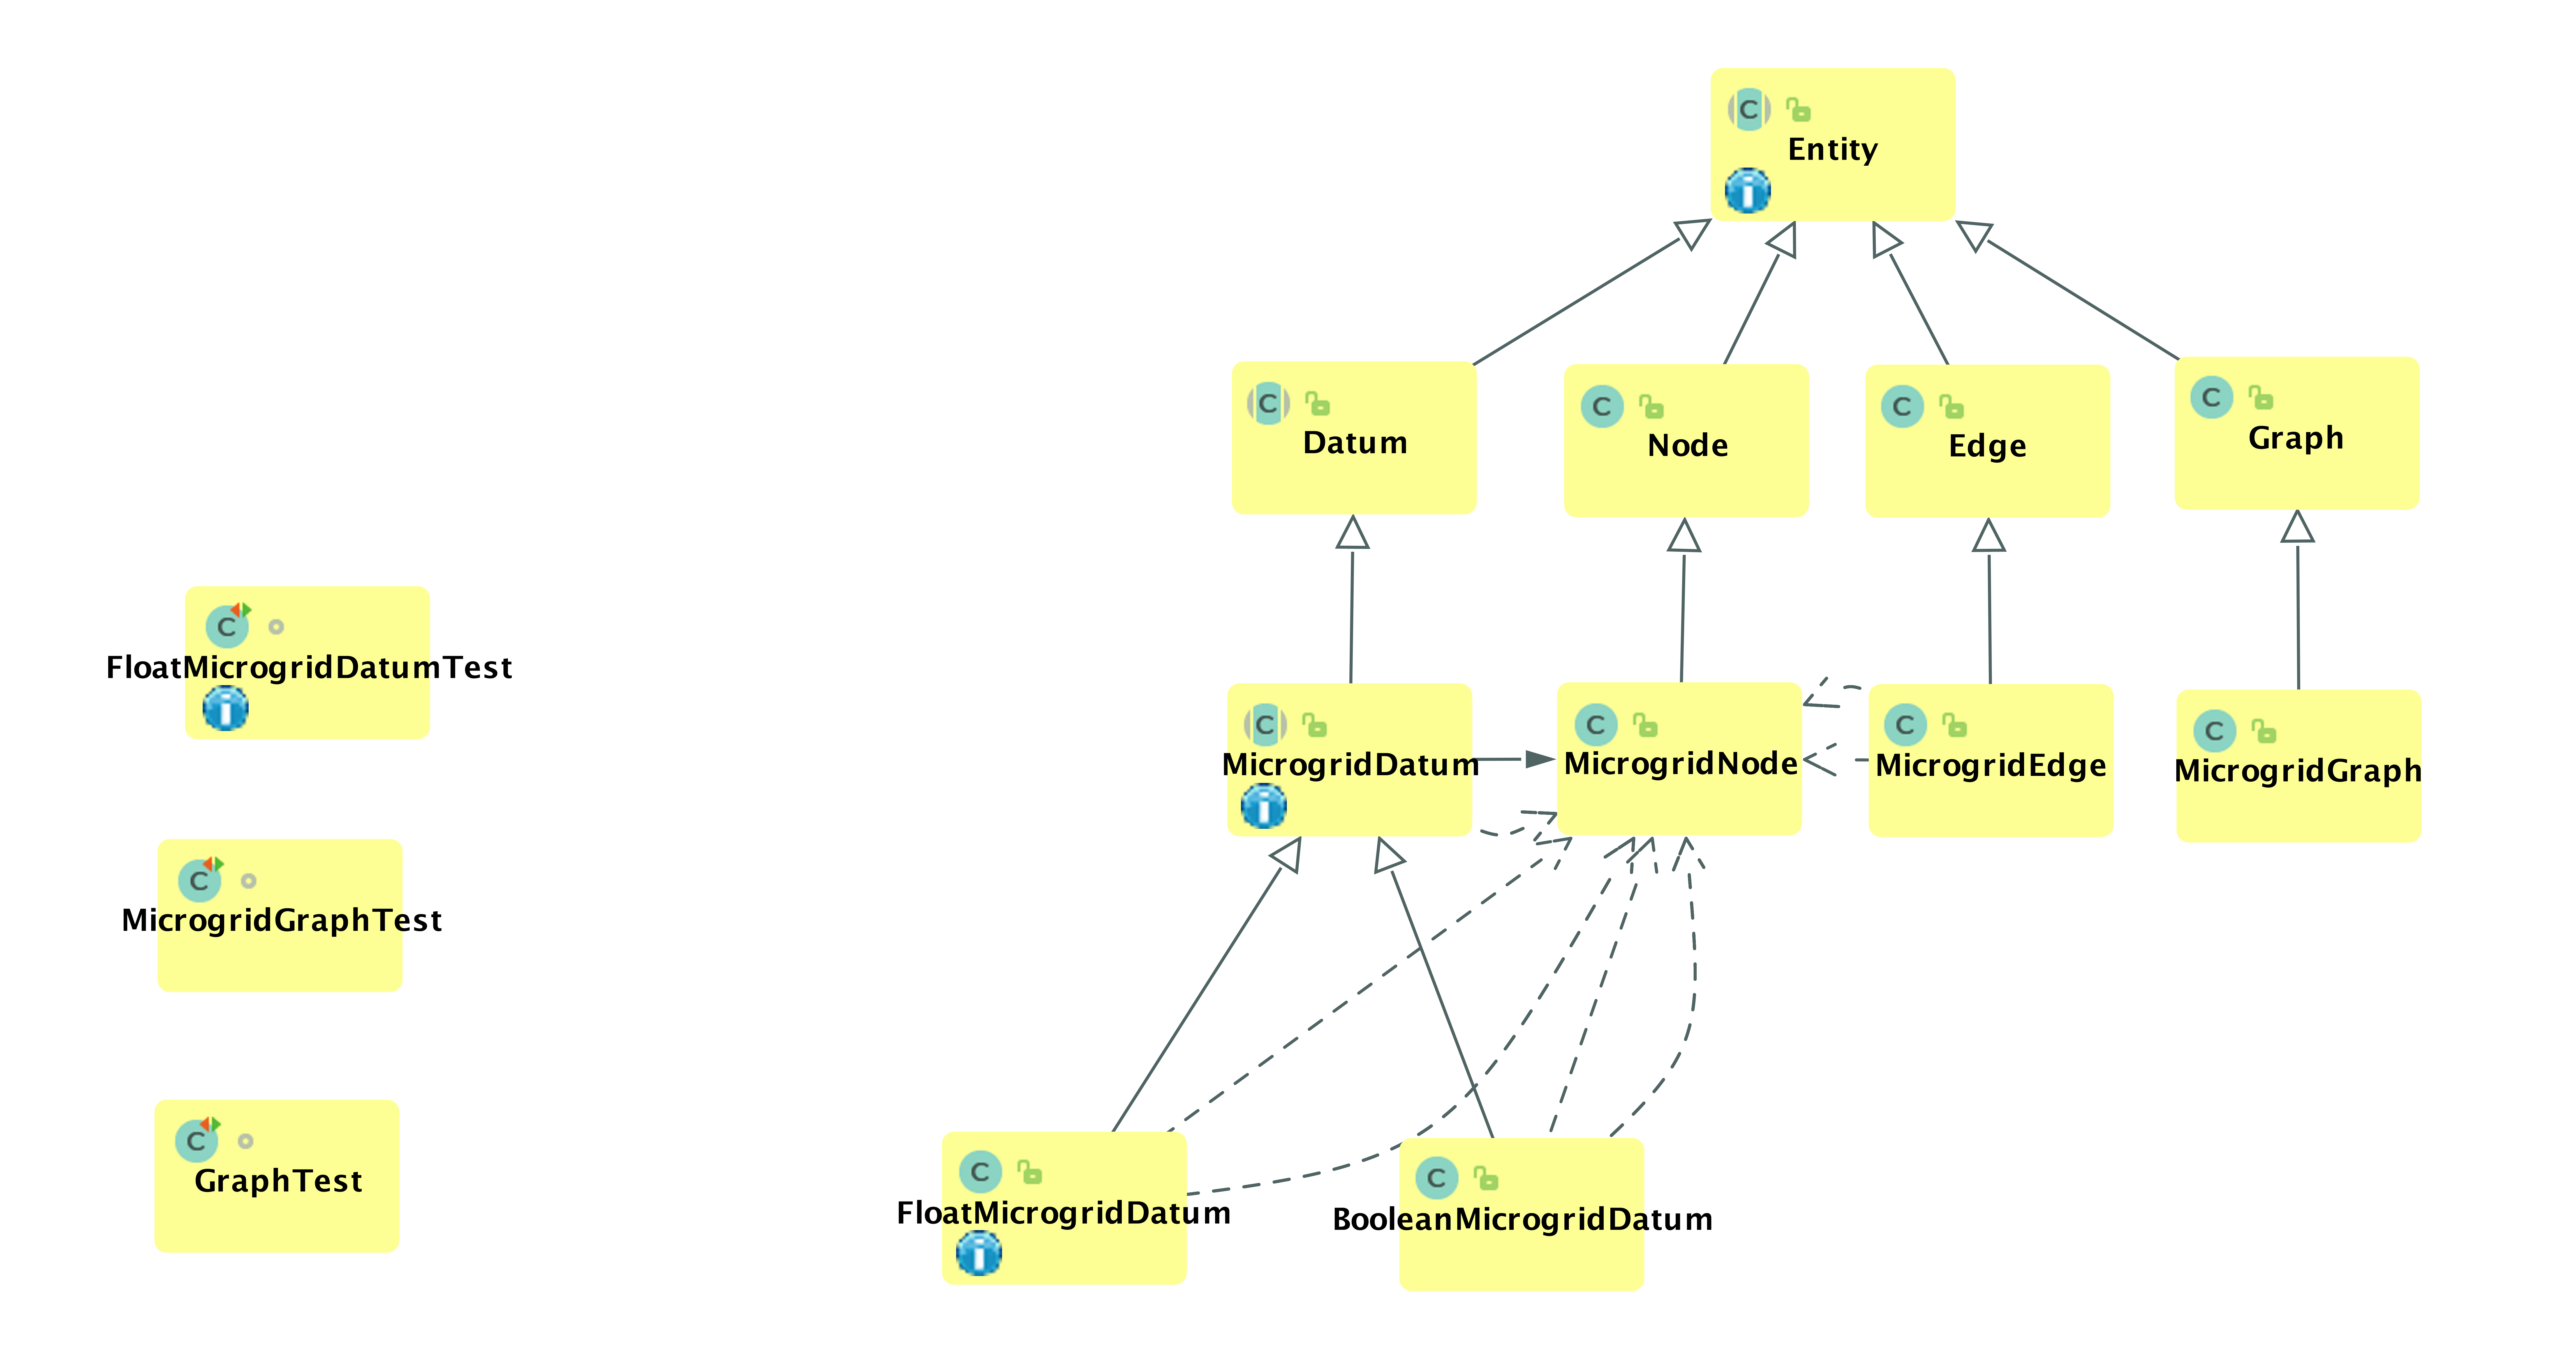
\includegraphics[width=\textwidth]{dataPackageClassDiagram.png}

The goal of this model is to accurately represent a microgrid system for the purpose of developing and implementing control systems. It should be trivial to transform and to transmit this data about a system via networks. The model was developed as a reference implementation in Java. JADE is used as a transport layer, so an additional set of classes "wraps" the data model. These classes form a JADE dialect.

Grid topology data is treated as a graph data structure. Each controller agent is responsible for sending its “subgraph” to the receiving agent. The receiving agent the combines all subgraphs it has received into a final graph. Grid topology will rarely change in production systems and will change fairly slowly in development. As a result, grid topology is considered “semi-permanent” when it is sent. Sender agents are expected to send grid topology on startup. This grid topology data is expected to carry an expiration date. This puts the responsibility for determining how often topology data should be updated in the hands of sender implementation agents. Sender agents should send updates of their grid topology to the receiving agents just before the previous set of topology expires.

Measurement data is assumed to constantly change. It is also assumed to exist at some point on the grid topology graph. Each measurement consists of a measurement type, grid location, and a measurement.

Another goal of the communication protocol is to avoid re-inventing the wheel. JADE provides a transport layer to send Java objects as messages between JADE agents. Thus, we use Jade’s Agent Identifier (AID) identification system for agents, all communication is implemented via JADE INFORM messages containing externalized Java objects. As a result, the remainder of this document will describe Java classes. All data will be wrapped in “Message” objects in order to separate message processing logic from data model. The data model should function independently of the messaging layer used to move it.

All data objects implement the Externalizable interface from the Java serialization library. Each class definition is responsible for representing its own state in an output stream. As a result, all objects are compatible with ObjectOutputStream serialization. However, this protocol does not use Java serialization. Java serialization includes more redundant class definition data than actual data we want to transmit. Instead, objects call writeExternal() directly with a reference to an object output stream. As a result, only field data is outputted. Jade inform messages contain a byte[] that is the result of this process. Standard ObjectOutputStream serialization will/should work with all objects. However, this is not recommended because the stream adds class descriptors that contain redundant data. This overhead would choke message processing.

A reference implementation is provided. The java classes in the packages data and message in the reference implementation serve as the official protocol specification. The remainder of this document serves as an overview. Inheritance relationships have been omitted for clarity in the descriptions in the following document. However, inheritance from basic data types (such as “Graph”) is implemented in the Java classes.


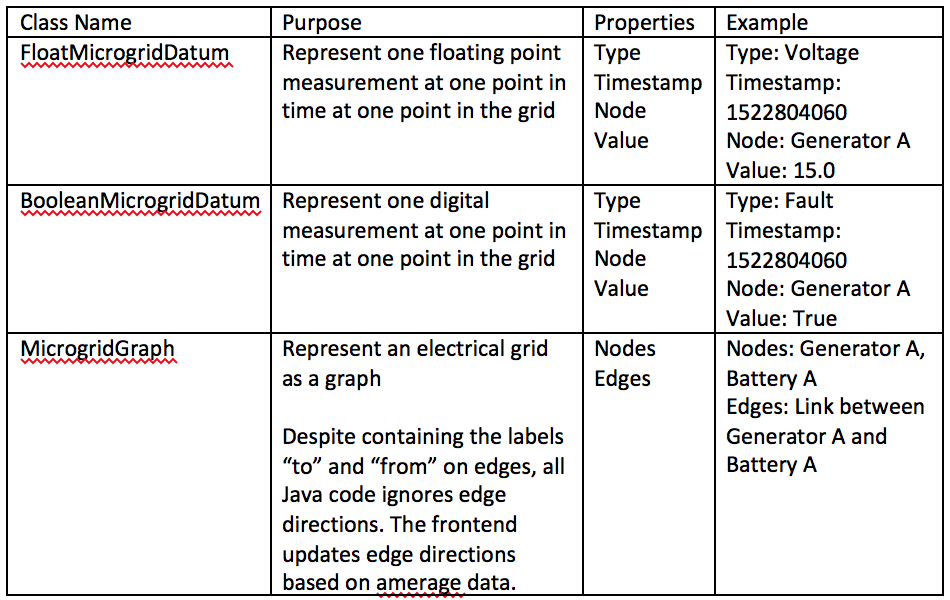
\includegraphics[width=\textwidth]{tableDataTypes.png}
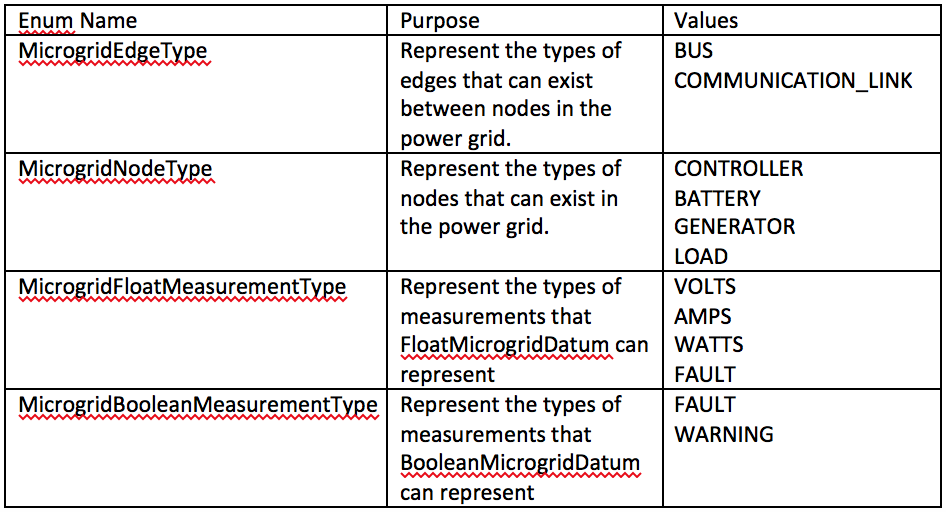
\includegraphics[width=\textwidth]{tableDataSubtypes.png}
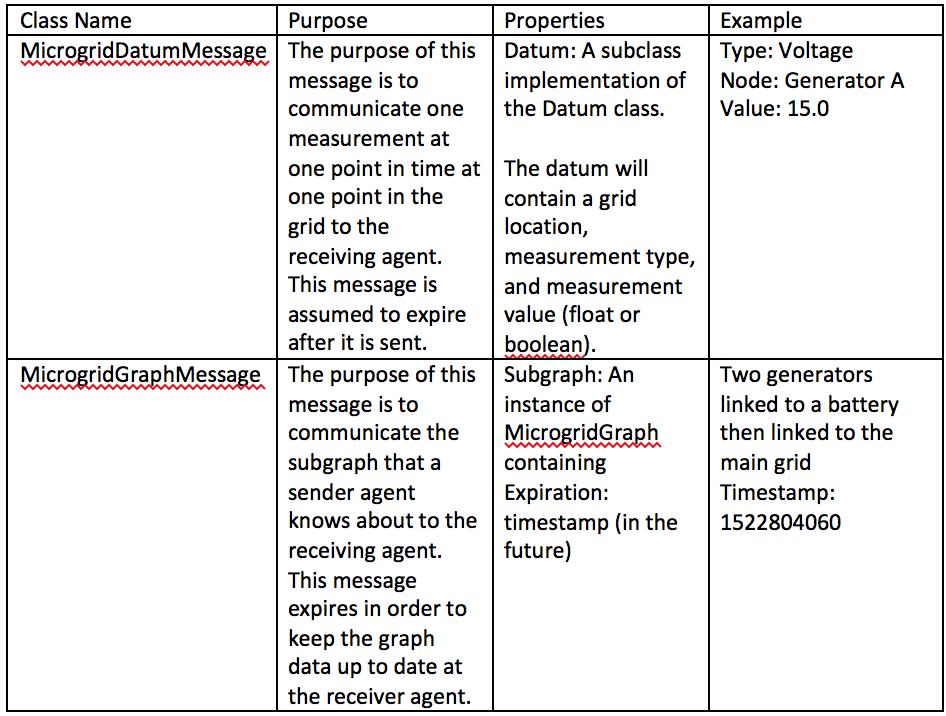
\includegraphics[width=\textwidth]{tableMessageTypes.png}

\subsection{Visualization}
Since the microgrid is represented in memory as a graph, representing the graph is a graph-drawing problem. A force-directed-layout can visualize even complicated grid systems. The reference implementation uses the JavaScript library Vis.JS to accomplish this.

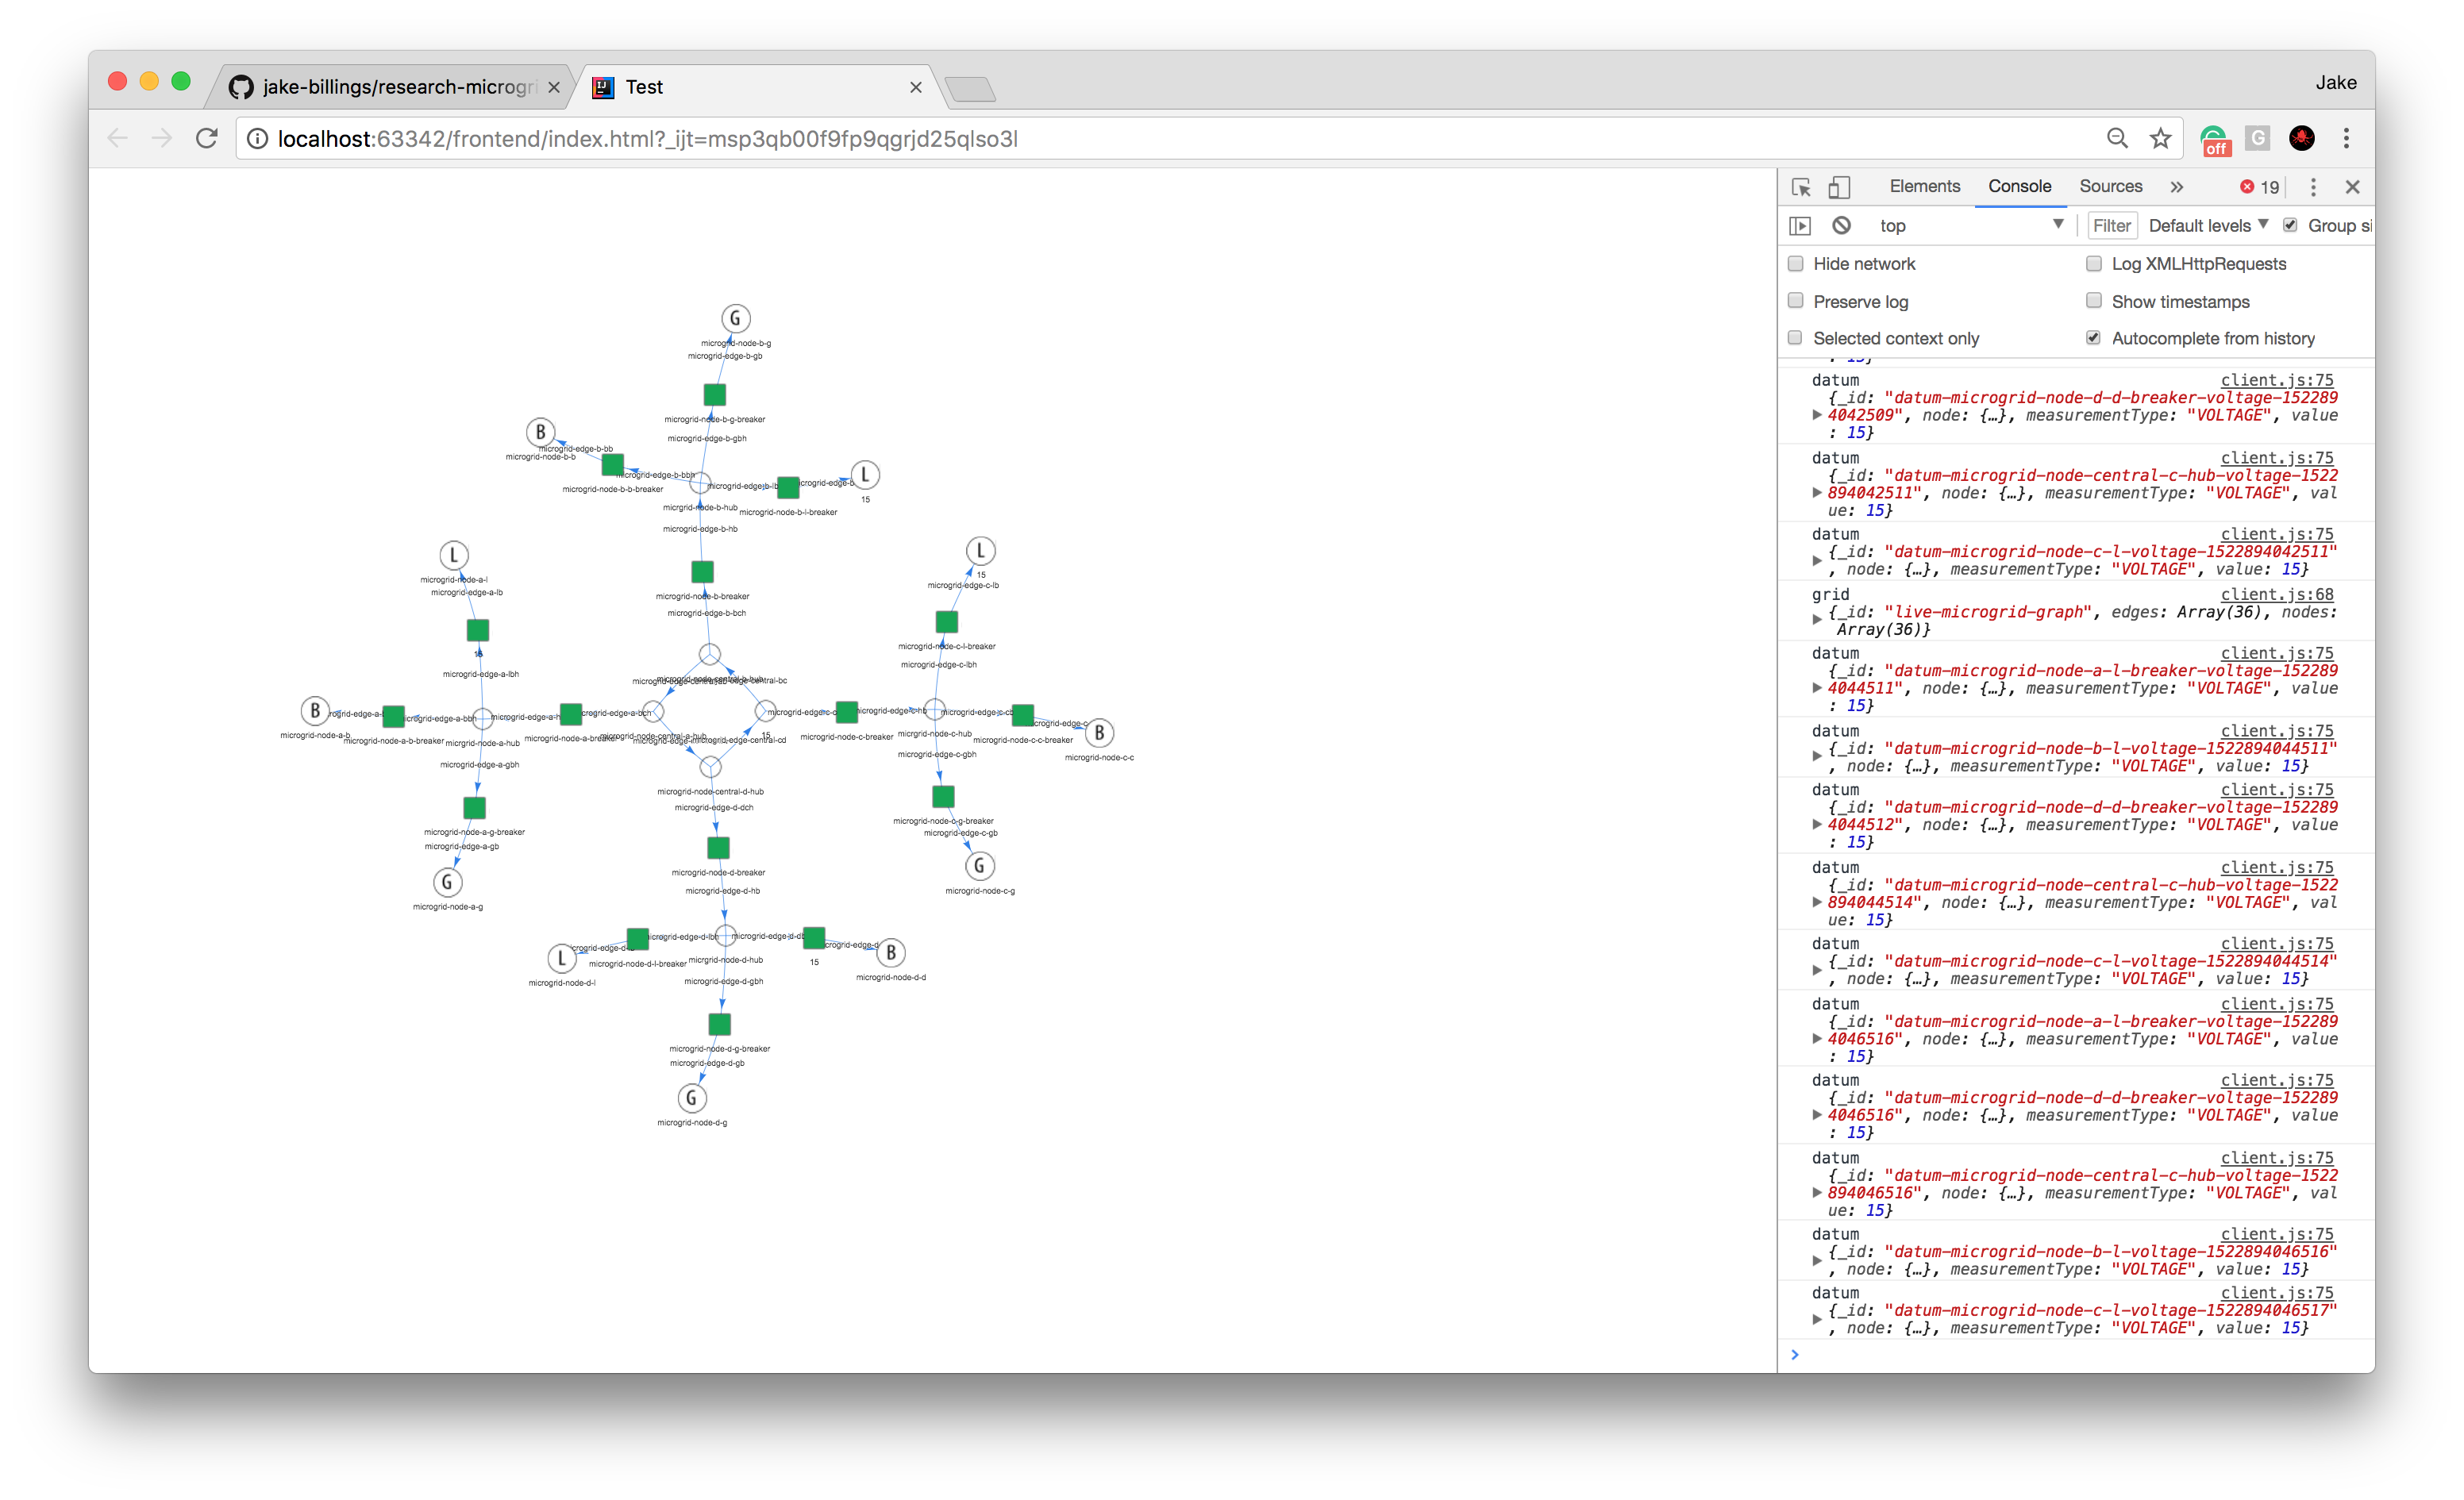
\includegraphics[width=\textwidth]{screenshots/preliminaryGraphRendering.png}

\section{Monitoring}
Theoritically, this data model could be implemented in any language to monitor any network. In this paper, I explore only the reference implementation.

\subsection{Implementation}
JADE is used to facilitate system design and communication. There are two types of agents in the reference implementation: Senders (subclasses of MicrogridSenderAgent) and Receivers (subclasses of MicrogridReceiverAgent). Senders accept data from hardware controllers, instantiate Java objects from the data model, and send them to a receiver agent. the MicrogridSenderAgent superclass contains queue management and ACL messaging code. The MicrogridReceiverAgent superclass is a fully-functional receiver agent. It keeps a copy of the most-up-to-date state of the microgrid in its memory and periodically sends snapshots of it an online monitoring tool via a WebSocket interface. DataLoggingMicrogridReceiverAgent demonstrates an agent that logs all data it receives to an SQL database using the Hibernate JPA implementation. Example, Dummy, and Functional agents are included for reference.

\end{document}